\chapter{Physikalischer Hintergrund}
%
\section{Standardmodell der Teilchenphysik}
%
Das Standardmodell (SM) der Teilchenphysik beschreibt den Aufbau der Materie, sowie ihre Wechselwirkung auf elemtarer Ebene. Sie stellt eine seit vielen Jahrzehnten bestehende und damit vielfältig getestete Theorie dar und unterliegt auch heute weiter regelmäßigen Tests.
Die Grundkonstituenten nach dem Standardmodell sind die drei Generationen von Quarks, sowie drei Generationen von Leptonen, wie sie unten aufgeführt sind.

\begin{figure}
  \centering
      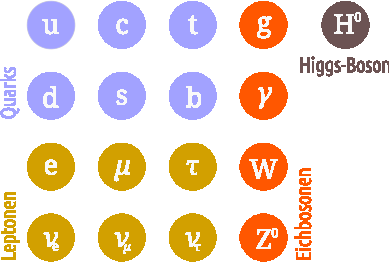
\includegraphics[width=0.6\textwidth]{content/SM.pdf}
  \caption{Die Elementarteilchen im Stadardmodell der Teilchenphysik.}
\end{figure}


Die Unterteilung in diese zwei Gruppen, sowie in die verschiedenen Generationen erfolgt über die Eigenschaften der Teilchen. Leptonen sind beispielsweise punktförmige ganzzahlig geladene Fermionen und Quarks solche mit $\sfrac{1}{3}$ beziehungsweise $\sfrac{2}{3}$ Ladung. Es gilt für diese Darstellung dass die Teilchenmassen zwischen den Generationen von links nach rechts zunehmen.\\
Im Standardmodell unterscheidet man zwischen drei Wechselwirkungen der Elementarteilchen untereinander: die starke Wechselwrikung zwischen farbgeladenen Teilchen, die schwache Wechselwirkung an welcher alle Elementarteilchen teilnehmen, sowie die elektromagetische Wechselwirkung, welcher nur elektrisch geladene Teilchen unterliegen. Die letzten beiden lassen sich im Rahmen des SM zur elektroschwachen Wechselwirkung vereinigen.
Die Farbladung in der starken Wechselwirkung beschreibt das Konzept einer Quantenzahl deren Existenz zur theoretischen Umsetzung des sogenannten \textit{confinement} dient. \textit{confinement} meint hierbei die Tatsache, dass alle elementaren Teilnehmer der starken Wechselwirkung nur in "farbneutralen" Zuständen frei existieren; freie Quarks lassen sich, da sie eine von null verschiedene Farbladung tragen also nicht frei beobachten.

Die Übertragung der Wechselwirkungen findet über sogenannte Bosonen statt. Bei der starken Wechselwirkung sind dies die acht verschiedenen Gluonen ($g$). Sie tragen eine Farbladung und einen ganzzahligen Spin $\hbar$ ($\hbar$: reduziertes Plancksches Wirkungsquantum). Die Austauschteilchen der elektroschwachen Wechselwirkung sind die Photonen ($\gamma$) für den elektromagnetischen Teil, sowie für die schwache Wechselwirkung das neutrale $\mathrm{Z}$-Boson und die geladenen $\mathrm{W^{\pm}}$-Bosonen.
